% Fragmento editable. Requiere tikz; no requiere bibliotecas adicionales.
% Esquema de componentes: no representa una realización ni un número de clientes.
% Ancho nominal: 0.96\textwidth, incluidos los bloques extremos.
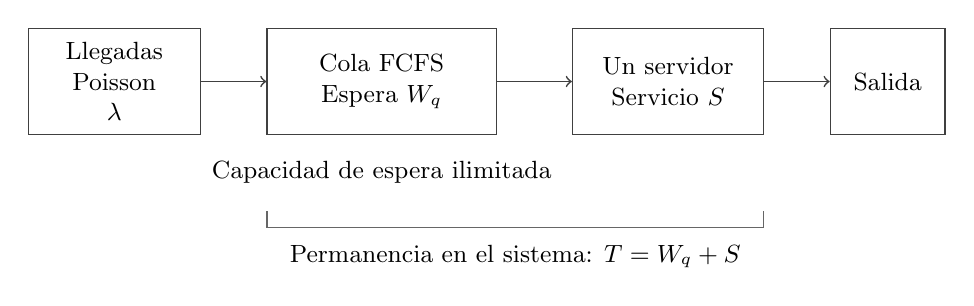
\begin{tikzpicture}[
  x=\textwidth,y=1cm,font=\small,
  bloque/.style={draw=black!75,fill=white,line width=0.5pt,
    align=center,inner sep=0pt,minimum height=1.35cm},
  flujo/.style={->,draw=black!75,line width=0.6pt}
]
  \node[bloque,text width=0.18\textwidth] (llegadas) at (0.09,0)
    {Llegadas\\Poisson\\$\lambda$};
  \node[bloque,text width=0.24\textwidth] (cola) at (0.37,0)
    {Cola FCFS\\Espera $W_q$};
  \node[bloque,text width=0.20\textwidth] (servidor) at (0.67,0)
    {Un servidor\\Servicio $S$};
  \node[bloque,text width=0.12\textwidth] (salida) at (0.90,0)
    {Salida};
  \draw[flujo] (llegadas.east) -- (cola.west);
  \draw[flujo] (cola.east) -- (servidor.west);
  \draw[flujo] (servidor.east) -- (salida.west);
  \node[align=center] at (0.37,-1.15) {Capacidad de espera ilimitada};
  \draw[draw=black!60,line width=0.45pt]
    (0.25,-1.65) -- (0.25,-1.85) -- (0.77,-1.85) -- (0.77,-1.65);
  \node[align=center,anchor=north] at (0.51,-1.95)
    {Permanencia en el sistema: $T=W_q+S$};
\end{tikzpicture}
